\documentclass{article}%standalone can be used
\usepackage{tikz}
\usetikzlibrary{shapes.geometric}

\begin{document}

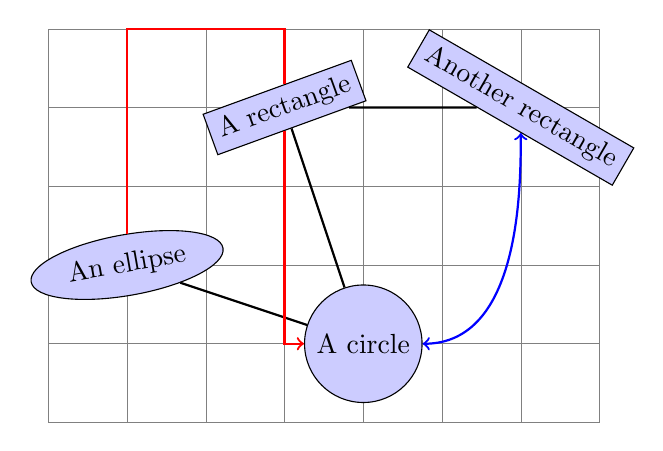
\begin{tikzpicture}[fill=blue!20] 
  \draw[style=help lines] (-1,-2) grid (6,3); 
  \path (0,0)  node(a) [ellipse,rotate=10,draw,fill]    {An ellipse} 
        (3,-1) node(b) [circle,draw,fill]               {A circle} 
        (2,2)  node(c) [rectangle,rotate=20,draw,fill]  {A rectangle} 
        (5,2)  node(d) [rectangle,rotate=-30,draw,fill] {Another rectangle}; 
  \draw[thick] (a) -- (b) -- (c) -- (d); 
  \draw[thick,red,->] (a) |- +(1,3) -| (c) |- (b); 
  \draw[thick,blue,<->] (b) .. controls +(right:2cm) and +(down:1cm) .. (d); 
\end{tikzpicture}
\end{document}
